\section{Open Job Shop Problem}
\subsection{Introduction}
\begin{frame}
  \frametitle{Problem definition}

  \begin{itemize}
    \item $m$ \textbf{jobs} have to processed by $n$ \textbf{machines}
    \item A job $i$ stays on a machine $j$ for an \textbf{operation} with start time $t_{ij}$ and duration $d_{ij}$
    \item The order in which a job is passed from machine to machine can be chosen arbitrarily.
  \end{itemize}

  Goal: \textbf{minimize} the total \textbf{makespan}, i.e. the time at which the last machine finishes its last operation.

 	

\end{frame}

\begin{frame}
	\frametitle{Example}
	
	\begin{columns}[c]
		\column{.4\linewidth}

Valid schedule for a 3x3-problem (3 jobs, 3 machines)

\textbf{makespan:} 23, matches lower bound

		\column{.6\linewidth}
\begin{figure}
	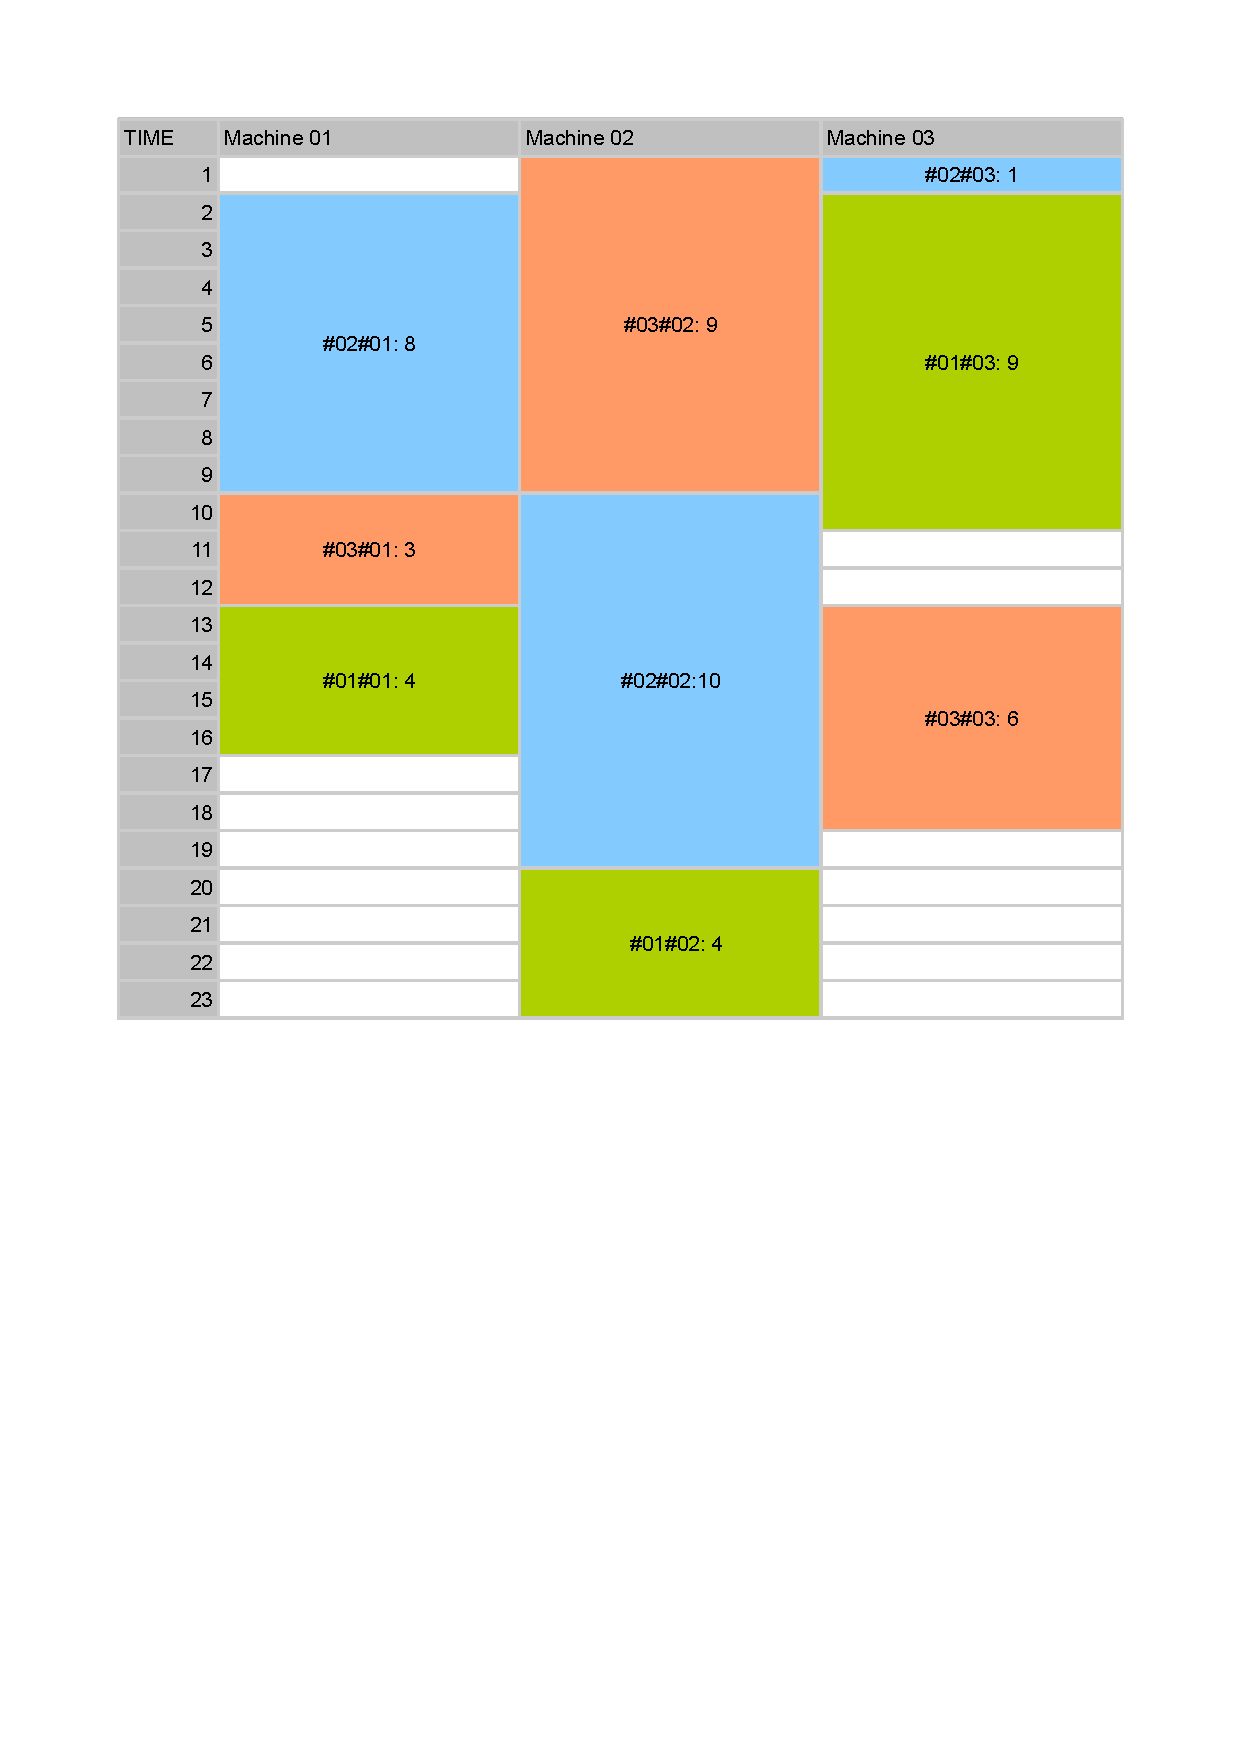
\includegraphics[width=\linewidth]{example-schedule.pdf}
	
\end{figure}
\end{columns}
	
\end{frame}

\subsection{Algorithms}
\begin{frame}
  \frametitle{Permutation Genetic Algorithm}


\end{frame}

\begin{frame}
  \frametitle{Hybrid Genetic Algorithm}
\end{frame}

\begin{frame}
  \frametitle{Selfish Gene Algorithm}
\end{frame}

\begin{frame}
  \frametitle{Other approaches}
\end{frame}